\clearpage
\section{基于最小包容原则、多维标度法和K均值聚类的聚类模型}
\subsection{模型的建立}
\subsubsection{最小包容原则}
\begin{figure}[htbp]
	\centering
	\caption{信号源运动时空轨迹}\label{信号源运动时空轨迹}
	\includegraphics[width=12cm]{move.eps}
\end{figure}
\par 可以看到最右边的点集中有8种R。根据抽屉原理至少有3艘船位置相近。需要通过聚类进一步细分。
\\\indent 先将近似线性的点集降维成点。将直线段降维成点的方法很多,但本题对信号源的聚类有特殊的条件。
\begin{description}
	\item[距离条件]属于同一船舶的信号源的时空距离应始终较小。
	\item[平行度条件]属于同一船舶的信号源运动的时空轨迹应该相互平行。
\end{description}
\par 根据以上2个条件,选择能共同衡量这2个条件符合程度的指标——最小包容圆柱直径对数据降维。
\\\indent 选择最小包容区域的形状为圆柱。因为理想情况下船舶做匀速直线运动,信号源运动时空轨迹近似为直线。当2个信号源完全重合时最小包容圆柱直径为0;当2个信号源完全平行但间距过大时,最小包容圆柱直径随间距增大而增大;当2个信号源间距为0但相交时,最小包容圆柱直径为随交角和信号源运动轨迹长度增大而增大。因此最小包容圆柱直径为与平行度和间距正相关的函数,圆柱直径越小,两信号源属于同一船舶概率越大。
\\\indent 对于关系不同的直线段,求解最小包容圆柱直径的算法如下。
\begin{figure}[htbp]
	\centering
	\begin{minipage}[htbp]{4cm}
		\centering
		\caption{平行}
		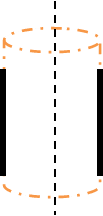
\includegraphics[height=4cm]{parallel.png}
	\end{minipage}
	\begin{minipage}[htbp]{4cm}
		\centering
		\caption{相交}
		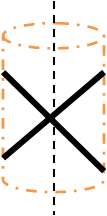
\includegraphics[height=4cm]{intersect.png}
	\end{minipage}
	\begin{minipage}[htbp]{5cm}
		\centering
		\caption{异面}
		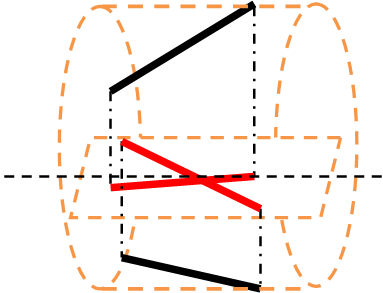
\includegraphics[height=4cm]{skew.png}
	\end{minipage}
\end{figure}
\par 最小包容圆柱以虚线为中心轴。对于平行和相交,虚线为与直线段交角较小的对称轴。对于异面,平面为与两直线都平行且距离相等的平面,红线是黑线在平面上的投影,虚线为与红线段交角较小的对称轴。
\subsubsection{多维标度法}
记\(d(r_k,r_l)\)为信号源\(r_k,r_l\)的最小包容圆柱直径。称\(d\)为直径函数。注意到求出的直径函数\(d\)符合正定性、对称性和Minkowski\index{Minkowski}三角不等式,可以作为点的距离函数。
\begin{description}
	\item[正定性]函数值非负,当且仅当自变量的2个分量相等时取0。\par
	\begin{align}
		&	d(r_k,r_l)\geqslant0		\\
		&	d(r_k,r_l)=0\iff k=l
	\end{align}
	\item[对称性]交换自变量的2个分量,函数值不变。\par
	\begin{align}
		d(r_k,r_l)=d(r_l,r_k)
	\end{align}
	\item[Minkowski三角不等式]\par
	\begin{align}
		d(r_j,r_k)+d(r_k,r_l)\geqslant d(r_j,r_l)
	\end{align}
\end{description}
\begin{align}
	&	G=(V,E,w)						\\
	&	V=\{v_k|k=1..K\}					\\
	&	E=V^2=\{(v_k,v_l)|k,l=1..K\}			\\
	&	\forall k,l=1..K,w(v_k,v_l)=d(r_k,r_l)
\end{align}
\par\(K\)为信号源的个数,也是点的个数。\(G\)是赋权图,\(V\)是点集,\(E\)是边集,\(w\)是权,也是边长。每2个点的距离就是信号源两两的最小包容圆柱直径。每个点都与一个信号源一一映射,每个点集也与一个信号源集一一映射,记这2个映射的并为\(f\)。
\begin{align}
	&	\forall k=1..K,f(v_k)=r(k)				\\
	&	\forall v_k\in T,r_k\in S,k=1..K,f(T)=S
\end{align}
\par 利用多维标度法根据边长作出求出点的相对位置。对该图做聚类即为对信号源做聚类。属于同一类的信号源属于同一艘船。
\subsubsection{K均值聚类}
属于同一艘船舶的信号源有如下约束条件:
\begin{description}
	\item[信号源数量条件]每艘船舶能有最多3个R、1个L1、1个L2和1个A;
	\item[安全条件]船舶航行时为了避免碰撞应保持安全间距\cite{safe} 。即类与类的距离应尽可能的远。
\end{description}
\par 定义类与类的距离为两集合中距离最近的两点的距离。
\begin{align}
	d(A,B)=\min\limits_{a\in A,b\in B}d(a,b)
\end{align}
\par 最优聚类为满足以下条件的聚类。
\begin{align}
	&	\max F(\mathscr{T})	\\
	&	\mathrm{s.t.}
	\begin{cases}
		F(\mathscr{T})=\min\limits_{T_k,T_l\in \mathscr{T},k\neq l}d(T_k,T_l)										\\
		\bigcup\limits_{T\in\mathscr{T}}T=V																\\
		\bigcup\limits_{T_k,T_l\in\mathscr{T}}T_k\cap T_l=\emptyset											\\
		\max\limits_{T\in\mathscr{T}}\mathrm{card}(\{v_k\in T|\mathrm{kind}(r_k)=\mathrm{R},r_k=f(v_k)\})	\leqslant3		\\
		\max\limits_{T\in\mathscr{T}}\mathrm{card}(\{v_k\in T|\mathrm{kind}(r_k)=\mathrm{L1},r_k=f(v_k)\})\leqslant1	\\
		\max\limits_{T\in\mathscr{T}}\mathrm{card}(\{v_k\in T|\mathrm{kind}(r_k)=\mathrm{L2},r_k=f(v_k)\})\leqslant1	\\
		\max\limits_{T\in\mathscr{T}}\mathrm{card}(\{v_k\in T|\mathrm{kind}(r_k)=\mathrm{A},r_k=f(v_k)\})	\leqslant1
	\end{cases}
\end{align}
\par\(\mathrm{kind}(r_k)\)是信号源\(r_k\)的种类。第1个条件为安全条件,第2、3个条件为聚类的定义,第4、5、6、7个条件为信号源数量条件。
\\\indent 聚类算法需要输入指定参数。
\begin{table}[htbp]
	\centering
	\caption{常见聚类算法}
	\begin{tabular}{ccc}
		\toprule
		算法名					&	参数	名		&	参数类型	\\
		\midrule
		K均值聚类				&	类数			&	正整数	\\
		层次聚类					&	合并分离系数	&	正实数	\\
		非参Bayes\index{Bayes}	&	先验概率		&	正实数	\\
		密度聚类					&	密度			&	正实数	\\
		\bottomrule
	\end{tabular}
\end{table}
\begin{enumerate}
	\item 参数可以先取极端值使得所有点聚成一类,必不满足信号源数量条件;
	\item 再调整参数到一个临界值,使所有类刚刚满足信号源数量条件;
	\item 再调整参数到另一个极端值使得所有点自成一类,但此时可能有2个相距较近的信号源分到了不同的船使得无法保证安全。
\end{enumerate}
\par 用暴力穷举搜索从临界值到第二个极端值中能满足约束条件的最优聚类。
\\\indent 经过比较我们选用K均值聚类。因为合并分离系数、先验概率和密度都是实数,暴力穷举运算量大且无法真正穷举完。而类数是整数,可以有效减小计算量。
\subsection{模型的求解}
易从\ref{信号源运动时空轨迹}图中看出信号源大体分为3类。为减轻运算量,可对信号源先聚成3类后分别分析。
\\\indent 下图是考察最右边也是最复杂的一类的结果。对8种R做了聚类。
\begin{figure}[htbp]
	\centering
	\begin{minipage}[htbp]{4cm}
		\centering
		\caption{聚为3类}
		\includegraphics[height=4cm]{3.eps}
	\end{minipage}
	\begin{minipage}[htbp]{4cm}
		\centering
		\caption{聚为4类}
		\includegraphics[height=4cm]{4.eps}
	\end{minipage}
	\begin{minipage}[htbp]{5cm}
		\centering
		\caption{聚为5类}
		\includegraphics[height=4cm]{5.eps}
	\end{minipage}
\end{figure}
\begin{table}[htbp]
	\centering
	\caption{聚类比较}
	\begin{tabular}{cc}
		\toprule
		类数		&	最小安全距离/经纬度	\\
		\midrule
		3		&	1.02E+00				\\
		4		&	1.01E-02				\\
		5		&	1.06E-02				\\
		\bottomrule
	\end{tabular}
\end{table}
\par 一共有6艘船。属于同一艘船舶的信号源如下。
\begin{table}[htbp]
	\centering
	\caption{聚类结果}\small
	\begin{tabular}{ccccccc}
		\toprule
		R类信号源1         & R类信号源2   & R类信号源3         & LI1类信号源 & L2类信号源 & A类信号源  	&	信号源到聚类中心的平均距离	\\
		\midrule
		112 & -     & -     & 241 & 253 &   -  & 0.040646 \\
		156 & -     & -     & -      & -      &   -  & 0        \\
		196 & 439 & 472 & 524 & -      &  -   & 0.003434 \\
		261 & 298 & 392 & 379 & -      &  -  & 0        \\
		540   & 572   & 625   &   -     &    -    &   -  &   0.027546       \\
		672   &  -     &   -    &    -    &   -     & 671 & 	0.004168	\\ 
		\bottomrule
	\end{tabular}
\end{table}
\par 信号源到聚类中心的平均距离可以用来衡量同一类信号源的集中程度。
